% ============================================================
% GP-109 Research Paper — LaTeX Source
% Title: Can an AI Explanation Be Misused?
%        Testing Whether SHAP and LIME Help Patients Game
%        a Clinical Diabetes Risk Model
%
% Target venue: FAccT 2028 / AIES 2028
% Template: ACM Conference Proceedings
%
% Numbers in this file come from the v3 re-run (results/tables/*).
% Build from the paper/ folder:
%   pdflatex main && bibtex main && pdflatex main && pdflatex main
% ============================================================

\documentclass[sigconf,nonacm]{acmart}

% ---- Packages ------------------------------------------------
\usepackage{booktabs}       % professional tables
\usepackage{microtype}      % better typography
\usepackage{graphicx}       % figures
\usepackage{subcaption}     % subfigures
\usepackage{amsmath}        % math
\usepackage{xcolor}
\usepackage{multirow}
\usepackage{array}
\usepackage{cleveref}       % \cref (acmart already loads hyperref)

% Narrow two-column layout: allow a little extra inter-word stretch
% instead of letting long words or citations stick into the margin.
\setlength{\emergencystretch}{1.5em}

% ---- Metadata ------------------------------------------------
\title{Can an AI Explanation Be Misused? Testing Whether SHAP and LIME
       Help Patients Game a Clinical Diabetes Risk Model}

\author{Akash Singh}
\affiliation{%
  \institution{Delhi Technological University}
  \city{Delhi}
  \country{India}
}
\email{akash@dtu.ac.in}

\author{Aditya Jha}
\affiliation{%
  \institution{Delhi Technological University}
  \city{Delhi}
  \country{India}
}
\email{aditya@dtu.ac.in}

\author{Akshat Kumar}
\affiliation{%
  \institution{Delhi Technological University}
  \city{Delhi}
  \country{India}
}
\email{akshat@dtu.ac.in}

% ============================================================
\begin{document}

% ---- Abstract -----------------------------------------------
\begin{abstract}
Explainable AI (XAI) methods such as SHAP and LIME are increasingly
required by regulation to accompany machine learning predictions in
healthcare. A concern is that feature attributions may also serve as
instructions for gaming the model---telling a patient which
self-reported inputs to change for a better risk score---so that
explanations should be withheld. But a patient can also simply try
different answers and watch the score move. We compare these two
strategies on a diabetes risk model trained on NHANES public health
survey data, where height and weight are recorded both as
self-reported and as measured by a nurse while the diabetes label
comes from a blood test (HbA1c). Lies are restricted to the size and
direction of real self-reporting errors observed in NHANES. We train
four models---Random Forest and Logistic Regression, each with
nurse-measured or self-reported height/weight---and measure the
\emph{explanation equivalence} $N^*$: how many blind attempts give the
same mean score reduction as one explanation-guided lie. In a
pre-registered confirmatory test on the NHANES 2021--2023 cycle
($n=1{,}126$ test patients), $N^* = 1.42$ (95\% CI 1.21--1.62) for the
primary configuration (Random Forest with SHAP) and 0--1.42 across all
configurations: one explanation is worth about one or two ordinary
attempts at the model.  An exploratory analysis of 2017--2018 and a
second dataset (BRFSS, 253{,}680 respondents) agree ($N^* = 0$, upper
95\% bounds $\le 1.2$).
Random-Forest lies suggested by an explanation often raise the score
instead.  The model that uses nurse-measured inputs cannot be gamed and
is as accurate.  Withholding explanations is therefore not an effective
safeguard; verifying self-reported inputs is.  We disclose that our
first pre-registered test set was examined before the analysis was
corrected, and release code, data pipeline and both analysis plans.
\end{abstract}

% ---- CCS Concepts / Keywords --------------------------------
\begin{CCSXML}
<ccs2012>
  <concept>
    <concept_id>10010147.10010257.10010293</concept_id>
    <concept_desc>Computing methodologies~Machine learning</concept_desc>
    <concept_significance>500</concept_significance>
  </concept>
  <concept>
    <concept_id>10003456.10003462</concept_id>
    <concept_desc>Social and professional topics~Medical records</concept_desc>
    <concept_significance>300</concept_significance>
  </concept>
</ccs2012>
\end{CCSXML}

\ccsdesc[500]{Computing methodologies~Machine learning}
\ccsdesc[300]{Social and professional topics~Medical records}

\keywords{explainability, SHAP, LIME, adversarial, gaming, diabetes,
          NHANES, clinical AI, transparency, fairness}

\maketitle

% ============================================================
\section{Introduction}
% ============================================================

The deployment of machine learning models in high-stakes clinical
settings has prompted widespread calls for transparency.  Regulations
such as the EU AI Act and GDPR's ``right to explanation'' push
developers to provide explanations alongside predictions
\cite{goodman2017european}.  In diabetes risk prediction, a model
might inform a patient: ``Your risk score is 0.72. Your weight is the
most important contributing factor.''

This transparency creates a potential dual-use risk: the same
explanation that helps a clinician understand the model may help a
patient \emph{game} it by adjusting what they self-report.  A patient
told that weight is the top risk factor might under-report their weight
at the next visit.  If explanations act as instructions for cheating,
one response is to hide them.

\paragraph{Our Question.}
A patient does not need an explanation to game a model: they can try
a few different answers and keep the one with the best score.  The
relevant question is therefore not whether an explanation helps at
all, but whether it helps \emph{more than ordinary trial-and-error}.
If explanations add little over a few blind attempts, restricting them
is not an effective safeguard.  If they add a lot, the benefit of
transparency must be weighed against the gaming risk.

\paragraph{Contributions.}
\begin{enumerate}
  \item We introduce \emph{explanation equivalence} ($N^*$): the
        number of blind attempts required to achieve the same mean
        score reduction as one explanation-guided attempt.
  \item We bound the adversary's lies by \emph{real} self-reporting
        behaviour: NHANES records both self-reported and
        nurse-measured height and weight, so we take the size and
        direction of a realistic lie from the observed gap.
  \item We train two models that differ \emph{only} in whether
        height/weight are self-reported or measured, isolating the
        effect of input verification.
  \item We conduct a \emph{pre-registered} confirmatory evaluation of
        SHAP and LIME on an unseen NHANES cycle and find that, under
        realistic lies, one explanation is worth about one to two blind
        attempts ($N^* \le 1.42$), replicated on a second survey.
\end{enumerate}

% ============================================================
\section{Related Work}
% ============================================================

\paragraph{Explainability Methods.}
Local explanation methods such as LIME~\cite{ribeiro2016lime} and
SHAP~\cite{lundberg2017shap} produce feature attributions that
identify the most important inputs for a given prediction.  These
methods are increasingly embedded in clinical decision support
systems~\cite{adadi2018peeking}.  Explanations can look convincing
yet be disconnected from the model~\cite{adebayo2018sanity}, and
Bilodeau et al.~\cite{bilodeau2024impossibility} proved that for
broad model classes feature attributions can do no better than random
guessing at predicting how the model responds to a change in its
input---showing that a problem is possible, but not how large it is
in practice.

\paragraph{Adversarial XAI.}
Slack et al.~\cite{slack2020fooling} demonstrated that SHAP and LIME
can be manipulated at the \emph{model} level to produce misleading
explanations, and Bordt et al.~\cite{bordt2022posthoc} argue that
post-hoc explanations suit legal transparency rules poorly because
providers can manipulate them.  Our work is complementary: we study
gaming at the \emph{user} level, asking whether an honest model's
explanations help a user game their score.  Milli et
al.~\cite{milli2019model} showed that a few explanation queries can
replace many ordinary queries for reconstructing a model, and Shokri
et al.~\cite{shokri2021privacy} showed that explanations can leak
private training data; both concern the model or its data rather than
a patient changing their own answers.

\paragraph{Strategic Classification.}
Ghalme et al.~\cite{ghalme2021strategic} found that hiding the
decision rule usually does not help the decision-maker, and Hikri and
Rosenfeld~\cite{hikri2026ambiguous} extended this to partial
disclosure.  K\"{o}nig et al.~\cite{konig2023improvement} note that advice
can improve a prediction without improving the person, just as lying
about weight is not losing weight.  Unlike these works, we bound
manipulation by real human misreporting and compare explanations
against an equal-cost blind baseline.

\paragraph{Self-Reporting Bias.}
NHANES~\cite{johnson2014national} systematically collects both
self-reported and nurse-measured anthropometrics, enabling a direct
empirical measurement of how people misreport.

% ============================================================
\section{Problem Setup}
% ============================================================

\subsection{Threat Model}

We model an adversary (patient) who:
\begin{itemize}
  \item Receives a diabetes risk score $f(\mathbf{x}) \in [0,1]$ from
        a clinical AI system and wishes to lower it.
  \item Can change only \emph{self-reported} features
        $G = \{\text{height}, \text{weight}\}$; nurse-measured values
        and lab results cannot be changed.
  \item Lies only \emph{realistically}: in the direction people
        actually misreport, by at most the lie budget $B(g)$.
  \item Either receives one SHAP/LIME explanation, or receives none
        and makes $N$ blind attempts, keeping the best score.
\end{itemize}

\subsection{Realistic Lies}

For each gameable feature $g$, the lie budget is
\[
  B(g) = \text{Percentile}_{95}\bigl(|x_g^{\text{self}} - x_g^{\text{measured}}|\bigr),
\]
computed on the 2015--2016 development cycle:
$B(\text{height}) = 7.28\,\text{cm}$ and
$B(\text{weight}) = 8.96\,\text{kg}$.  People over-report height
(mean $+1.62$\,cm) and under-report weight (mean $-0.87$\,kg), so a
realistic lie \emph{increases} height or \emph{decreases} weight.
Each lie has a size drawn uniformly from $(0, B(g)]$; the same rule is
used by both strategies, so the explanation contributes only
\emph{information} (which feature, which direction), never a larger lie.

\subsection{Explanation Equivalence}

\begin{definition}[Explanation Equivalence $N^*$]
Let $R_{\text{exp}}$ be the score reduction from one
explanation-guided lie, averaged over patients, and let
$R_{\text{blind}}(N)$ be the reduction from the best of $N$ blind
lies, averaged over patients.  The \emph{explanation equivalence} is
\[
  N^* = \inf \{ N \geq 0 : R_{\text{blind}}(N) \geq R_{\text{exp}} \},
\]
estimated by linear interpolation on $N \mapsto R_{\text{blind}}(N)$ for
\[
  N \in \{1,2,3,5,10,15,20,30,50,100\}.
\]
$N^*=0$ if one explanation does no better than a single blind
attempt; $N^*=101$ if it beats 100 attempts (censored).
\end{definition}

This is the pre-registered primary metric: the average is taken over
patients \emph{before} interpolating.  As secondary metrics we also
report the per-patient $N^*$ distribution.

% ============================================================
\section{Methodology}
% ============================================================

\subsection{Dataset}

We use the NHANES public health survey~\cite{johnson2014national} and
merge the demographics (DEMO), body measures (BMX), weight history
questionnaire (WHQ), glycohaemoglobin (GHB), blood pressure (BPX),
smoking (SMQ), and physical activity (PAQ) files for the 2015--2016
(development), 2017--2018 (exploratory test) and August
2021--August 2023 (confirmatory test) cycles.  Refused and
don't-know codes are removed per variable as in the NHANES codebooks.
Retaining adults ($\geq$18 years) with complete records for both
feature sets gives 4{,}889 participants in 2015--2016 (12.4\% with
diabetes, HbA1c $\geq 6.5\%$~\cite{ada2023standards}) and 4{,}431 in
2017--2018 (13.6\%).  Within each cycle we use a stratified 80/20
split.  Models are \emph{retrained} on each cycle's training split with
the locked hyperparameters; only the lie budget (\S3.2) carries over
from 2015--2016.  The 2017--2018 evaluation uses its $n=887$ test
patients; because it was seen before the code was corrected
(\cref{sec:preregistration}), we treat it as \emph{exploratory} and
re-test the final analysis on the August 2021--August 2023 cycle, which
no one on the team had analysed (\emph{confirmatory};
\cref{sec:confirmatory}).  In that cycle systolic blood pressure is
measured with an oscillometric device (\texttt{BPXOSY1}) and vigorous
activity is derived from the redesigned activity question
(\texttt{PAD810Q} $>0$); both mappings were fixed before the data was
processed.

\paragraph{Supporting datasets.}  As planned, we use two UCI datasets.
UCI Heart Disease (Cleveland, 297 patients) serves as a hand-checkable
test of the code: with a logistic regression every risk score, SHAP
value, suggested lie and blind best-of-$N$ has a closed form, and the
pipeline reproduces all of them to machine precision.  The CDC Diabetes
Health Indicators dataset (BRFSS 2015, 253{,}680 respondents) is a
comparison: its BMI is computed from self-reported height and weight,
so it supports only a Model~B analysis, and its diabetes label is
itself self-reported.

\subsection{Models}

Each model uses seven features: age, sex, systolic blood pressure,
smoking (ever 100 cigarettes), vigorous recreational activity,
height, and weight.  \emph{Model A} uses nurse-measured height/weight;
\emph{Model B} uses the self-reported values; everything else is
identical.  We train a Random Forest (RF; 100 trees, maximum depth 10)
and a Logistic Regression (LR; standardised inputs) for each, with
balanced class weights to account for the 13\% prevalence
(\cref{tab:model_perf}).  On the 2017--2018 test set the models reach
AUC 0.77--0.80 and recall 0.69--0.78; Models A and B perform almost
identically.

\begin{table}[htbp]
  \centering
  \caption{Model Performance on NHANES 2017–2018 Test Set}
  \label{tab:model_perf}
  \small
  \begin{tabular}{lrrrrrrr}
    \hline
    Config & Input & Model & Accuracy & Precision & Recall & F1 & AUC-ROC \\
    \hline
    measured_rf & measured & RF & 0.7396 & 0.3007 & 0.686 & 0.4181 & 0.7981 \\
    measured_lr & measured & LR & 0.6652 & 0.2569 & 0.7686 & 0.3851 & 0.7734 \\
    reported_rf & reported & RF & 0.7407 & 0.3032 & 0.6942 & 0.4221 & 0.7933 \\
    reported_lr & reported & LR & 0.6685 & 0.2604 & 0.7769 & 0.39 & 0.7796 \\
    \hline
  \end{tabular}
\end{table}

\subsection{Explanations}

SHAP uses TreeExplainer for RF and LinearExplainer for LR (background:
a seeded random sample of 100 training rows).  LIME uses its tabular
explainer with 500 samples, its default discretisation of continuous
features, and all seven features shown.

\subsection{Adversarial Strategies}

\paragraph{Strategy 1 (Explanation-Guided).}
The patient requests one explanation and reads it the way it is
presented: features ranked by importance, each pushing the risk up or
down.  Going down the ranking, the patient takes the first gameable
feature whose risk-lowering direction is a realistic lie.  A SHAP
value measures a feature's effect relative to the average patient, so a
positive value (``your height raises your risk'') means moving the
value \emph{towards} the average and a negative one moving it further
away; LIME is read from its bins, e.g.\ raise the feature if the
explanation says ``\emph{weight $\le$ 62\,kg} raises risk''.  If no
realistic lie is suggested, the patient does not lie.  Otherwise they
lie once, with a size drawn as in \S3.2, and see the new score; like
the blind patient, who keeps the best score so far, they keep their
true answers if the lie made the score worse.

\paragraph{Strategy 2 (Blind Trial-and-Error).}
The patient makes $N$ sequential attempts.  Each picks a gameable
feature at random and lies in its realistic direction with a size
drawn as in \S3.2; the best score so far is kept.  The simulation runs
once up to $N=100$ and records the running best at each milestone, so
blind performance at large $N$ is not over-estimated.

Every patient has its own fixed random seed, so the SHAP and LIME
strategies, and Models A and B, are compared against identical blind
attempts.

\subsection{Statistical Analysis}

For each configuration we report $N^*$ with a 95\% CI from 1{,}000
bootstrap resamples of patients; a one-sided paired Wilcoxon
signed-rank test~\cite{wilcoxon1945individual} of the per-patient
explanation reduction against the best of $N=10$ blind attempts
($H_1$: explanation $>$ blind), with Holm-adjusted $p$-values across the
eight configurations as a secondary analysis; and Cohen's $d$.  For the
Model~A vs.~B comparison we report the AUC difference on the same test
patients with a paired bootstrap CI.  All models were
implemented with scikit-learn~\cite{pedregosa2011sklearn}.

\subsection{Pre-Registration and Deviations}
\label{sec:preregistration}

The analysis plan (hypotheses, metric, tests, interpretation
thresholds) was recorded as the git tag \texttt{v0.1-preregistration}
in the project repository on 28 October 2026, before the 2017--2018
data was processed.  \textbf{A first final run on the held-out data was
then made with the code as pre-registered, and its results were seen
before the analysis reported here.}  That run reported a per-patient
mean $N^*$ of 12.4 (95\% CI 10.5--14.5) for the primary configuration
(reported RF+SHAP) and 9.0--23.1 across all eight configurations,
which the pre-registered thresholds would classify as a moderate to
high threat.  A subsequent code review found implementation errors,
which we corrected so that the code matches the plan (primary $N^*$
computed from the averaged curve; the pre-registered 2015--2016 lie
budget; only self-reported values gameable, whereas the measured model
had been attacked through its nurse-measured inputs).  We also made
eight changes that \emph{deviate} from the plan: lies only in the
realistic direction; the same lie-size rule for both strategies
(previously the explanation always used the maximum lie while blind
attempts drew smaller ones); LIME showing all seven features
(previously five); balanced class weights; a random SHAP background;
per-patient random seeds; letting the explanation-guided patient
undo a lie that raised their score, as the blind patient implicitly
can; and reading the sign of a SHAP value relative to the average
patient (the earlier rule told, e.g., shorter-than-average patients to
claim to be even shorter; this bug was found by the UCI hand check).  Because these settings were chosen after a held-out result had
been seen, the 2017--2018 evaluation is not a clean confirmatory test,
and the change in conclusion should be read with that in mind.  Each
deviation is a documented switch in the code; the full timeline and the
first run's results are in \texttt{docs/preregistration\_disclosure.md}.

\paragraph{Confirmatory pre-registration.}\label{sec:confirmatory}
To obtain a clean test, the corrected analysis, including our predicted
result, was pre-registered again (\texttt{docs/analysis\_plan\_v5\_confirmatory.md},
git tag \texttt{v0.2-preregistration}, pushed to GitHub before the data
was processed) and run once, unchanged, on NHANES 2021--2023.

% ============================================================
\section{Results}
% ============================================================

\subsection{Reporting Gap}

\Cref{fig:gaps} shows self-reported minus nurse-measured values.  In
2017--2018, participants over-report height by $+1.69$\,cm on average
(SD 3.23) and under-report weight by $-0.67$\,kg (SD 4.84), closely
matching 2015--2016 ($+1.62$\,cm, SD 3.41; $-0.87$\,kg, SD 4.79).  The
95th-percentile gap in 2017--2018 (6.88\,cm, 9.32\,kg) is within
0.4\,cm and 0.4\,kg of the development budget we use.

\begin{figure}[t]
  \centering
  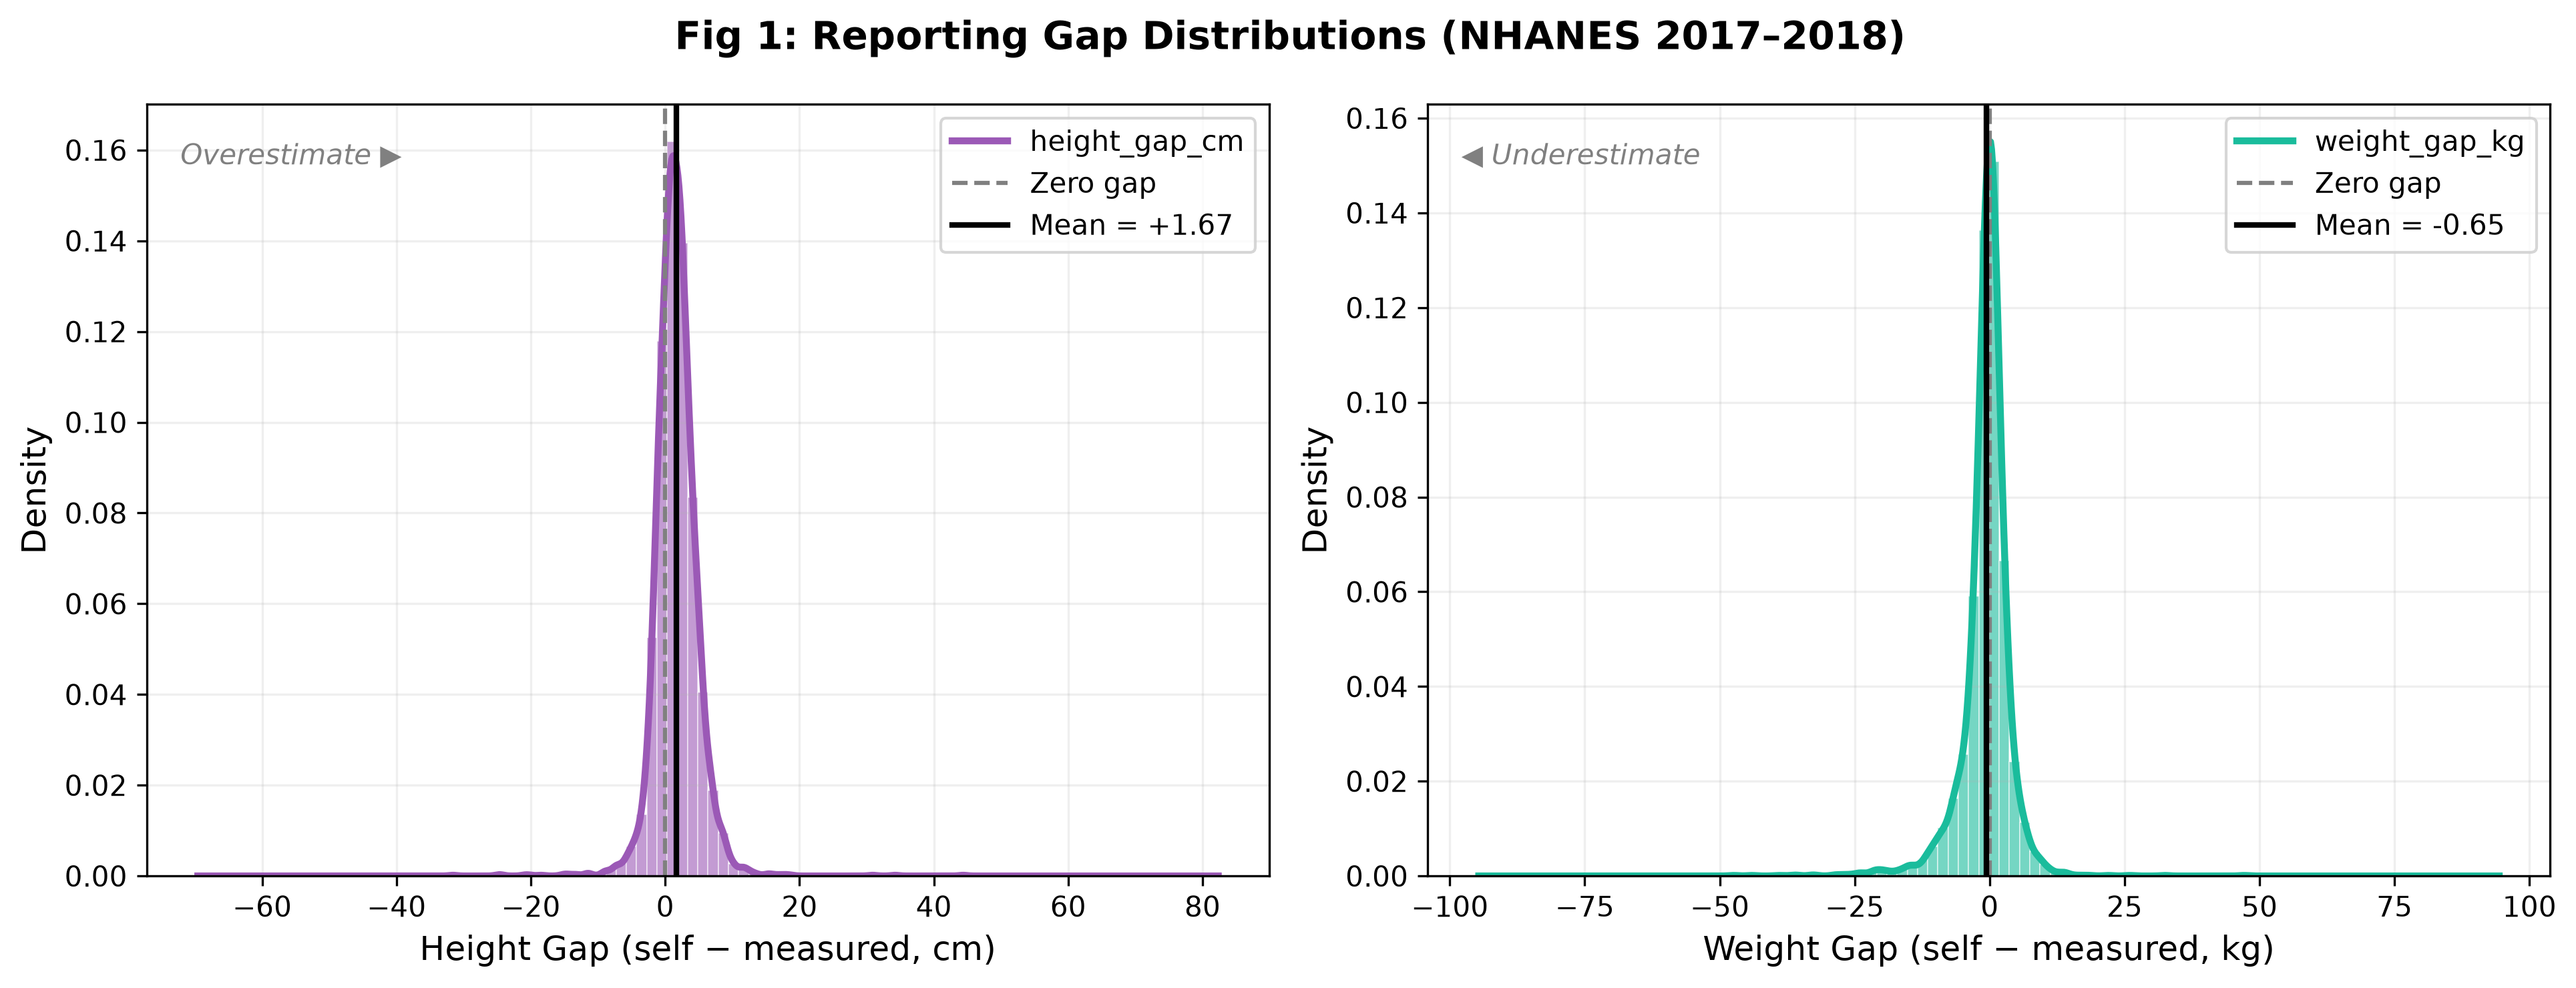
\includegraphics[width=\linewidth]{../results/figures/fig1_reporting_gaps.png}
  \caption{Self-reported minus nurse-measured height and weight
           (NHANES 2017--2018).  Height is over-reported and weight
           under-reported.}
  \label{fig:gaps}
\end{figure}

\subsection{Main Result: Explanation Equivalence (2017--2018, exploratory)}

On the 2017--2018 test set (exploratory, see \cref{sec:preregistration}),
$N^* = 0.0$ in all eight configurations (\cref{tab:main_results},
\cref{fig:main_result}); the primary configuration (Model B, RF+SHAP)
has a 95\% CI of 0.0--1.2.  For Model B, one explanation-guided lie
lowers the risk score by 0.018--0.024 on average, a single blind
attempt by 0.024--0.025, and the best of 10 blind attempts by
0.046--0.064 (\cref{tab:reductions}): an explanation is worth about one
ordinary attempt at the model, never more.  The confirmatory result on
2021--2023 is in \cref{sec:confirmatory-results}.

\begin{table*}[htbp]
  \centering
  \caption{Main Results: Explanation Equivalence $N^*$ Across All 8 Configurations}
  \label{tab:main_results}
  \small
  \resizebox{\ifdim\width>\linewidth\linewidth\else\width\fi}{!}{%
  \begin{tabular}{lrrrrrrrrr}
    \toprule
    Input & Model & Expl. & N patients & $N^*$ & 95\% CI & Per-patient mean $N^*$ & Per-patient median $N^*$ & \% Useless & \% Worth 10+ \\
    \midrule
    Reported & RF & SHAP & 887 & 0.0 & [0.00, 0.00] & 7.69 & 0.0 & 76.0\% & 8.7\% \\
    Reported & RF & LIME & 887 & 0.0 & [0.00, 0.00] & 7.07 & 0.0 & 73.8\% & 8.1\% \\
    Reported & LR & SHAP & 887 & 0.0 & [0.00, 0.00] & 2.58 & 0.0 & 66.4\% & 5.4\% \\
    Reported & LR & LIME & 887 & 0.0 & [0.00, 0.00] & 2.99 & 0.0 & 56.3\% & 6.1\% \\
    Measured & RF & SHAP & 887 & 0.0 & [0.00, 0.00] & 0.0 & 0.0 & 100.0\% & 0.0\% \\
    Measured & RF & LIME & 887 & 0.0 & [0.00, 0.00] & 0.0 & 0.0 & 100.0\% & 0.0\% \\
    Measured & LR & SHAP & 887 & 0.0 & [0.00, 0.00] & 0.0 & 0.0 & 100.0\% & 0.0\% \\
    Measured & LR & LIME & 887 & 0.0 & [0.00, 0.00] & 0.0 & 0.0 & 100.0\% & 0.0\% \\
    \bottomrule
  \end{tabular}%
  }
\end{table*}


\begin{table*}[htbp]
  \centering
  \caption{Mean risk-score reduction (0-1 scale): one explanation-guided lie vs. the best of N blind lies, and how often the explanation suggested no lie or a lie that raised the risk}
  \label{tab:reductions}
  \small
  \resizebox{\linewidth}{!}{%
  \begin{tabular}{lrrrrrrrr}
    \toprule
    Input & Model & Expl. & 1 explanation & 1 blind & 10 blind & 100 blind & \% no lie suggested & \% lie raised risk \\
    \midrule
    Reported & RF & SHAP & 0.0129 & 0.024 & 0.0638 & 0.0785 & 19.3\% & 23.0\% \\
    Reported & RF & LIME & 0.0117 & 0.024 & 0.0638 & 0.0785 & 3.3\% & 31.1\% \\
    Reported & LR & SHAP & 0.0176 & 0.0248 & 0.0457 & 0.0525 & 31.1\% & 0.0\% \\
    Reported & LR & LIME & 0.0223 & 0.0248 & 0.0457 & 0.0525 & 7.7\% & 0.0\% \\
    Measured & RF & SHAP & 0.0 & 0.0 & 0.0 & 0.0 & 100.0\% & 0.0\% \\
    Measured & RF & LIME & 0.0 & 0.0 & 0.0 & 0.0 & 100.0\% & 0.0\% \\
    Measured & LR & SHAP & 0.0 & 0.0 & 0.0 & 0.0 & 100.0\% & 0.0\% \\
    Measured & LR & LIME & 0.0 & 0.0 & 0.0 & 0.0 & 100.0\% & 0.0\% \\
    \bottomrule
  \end{tabular}%
  }
\end{table*}


\begin{figure*}[t]
  \centering
  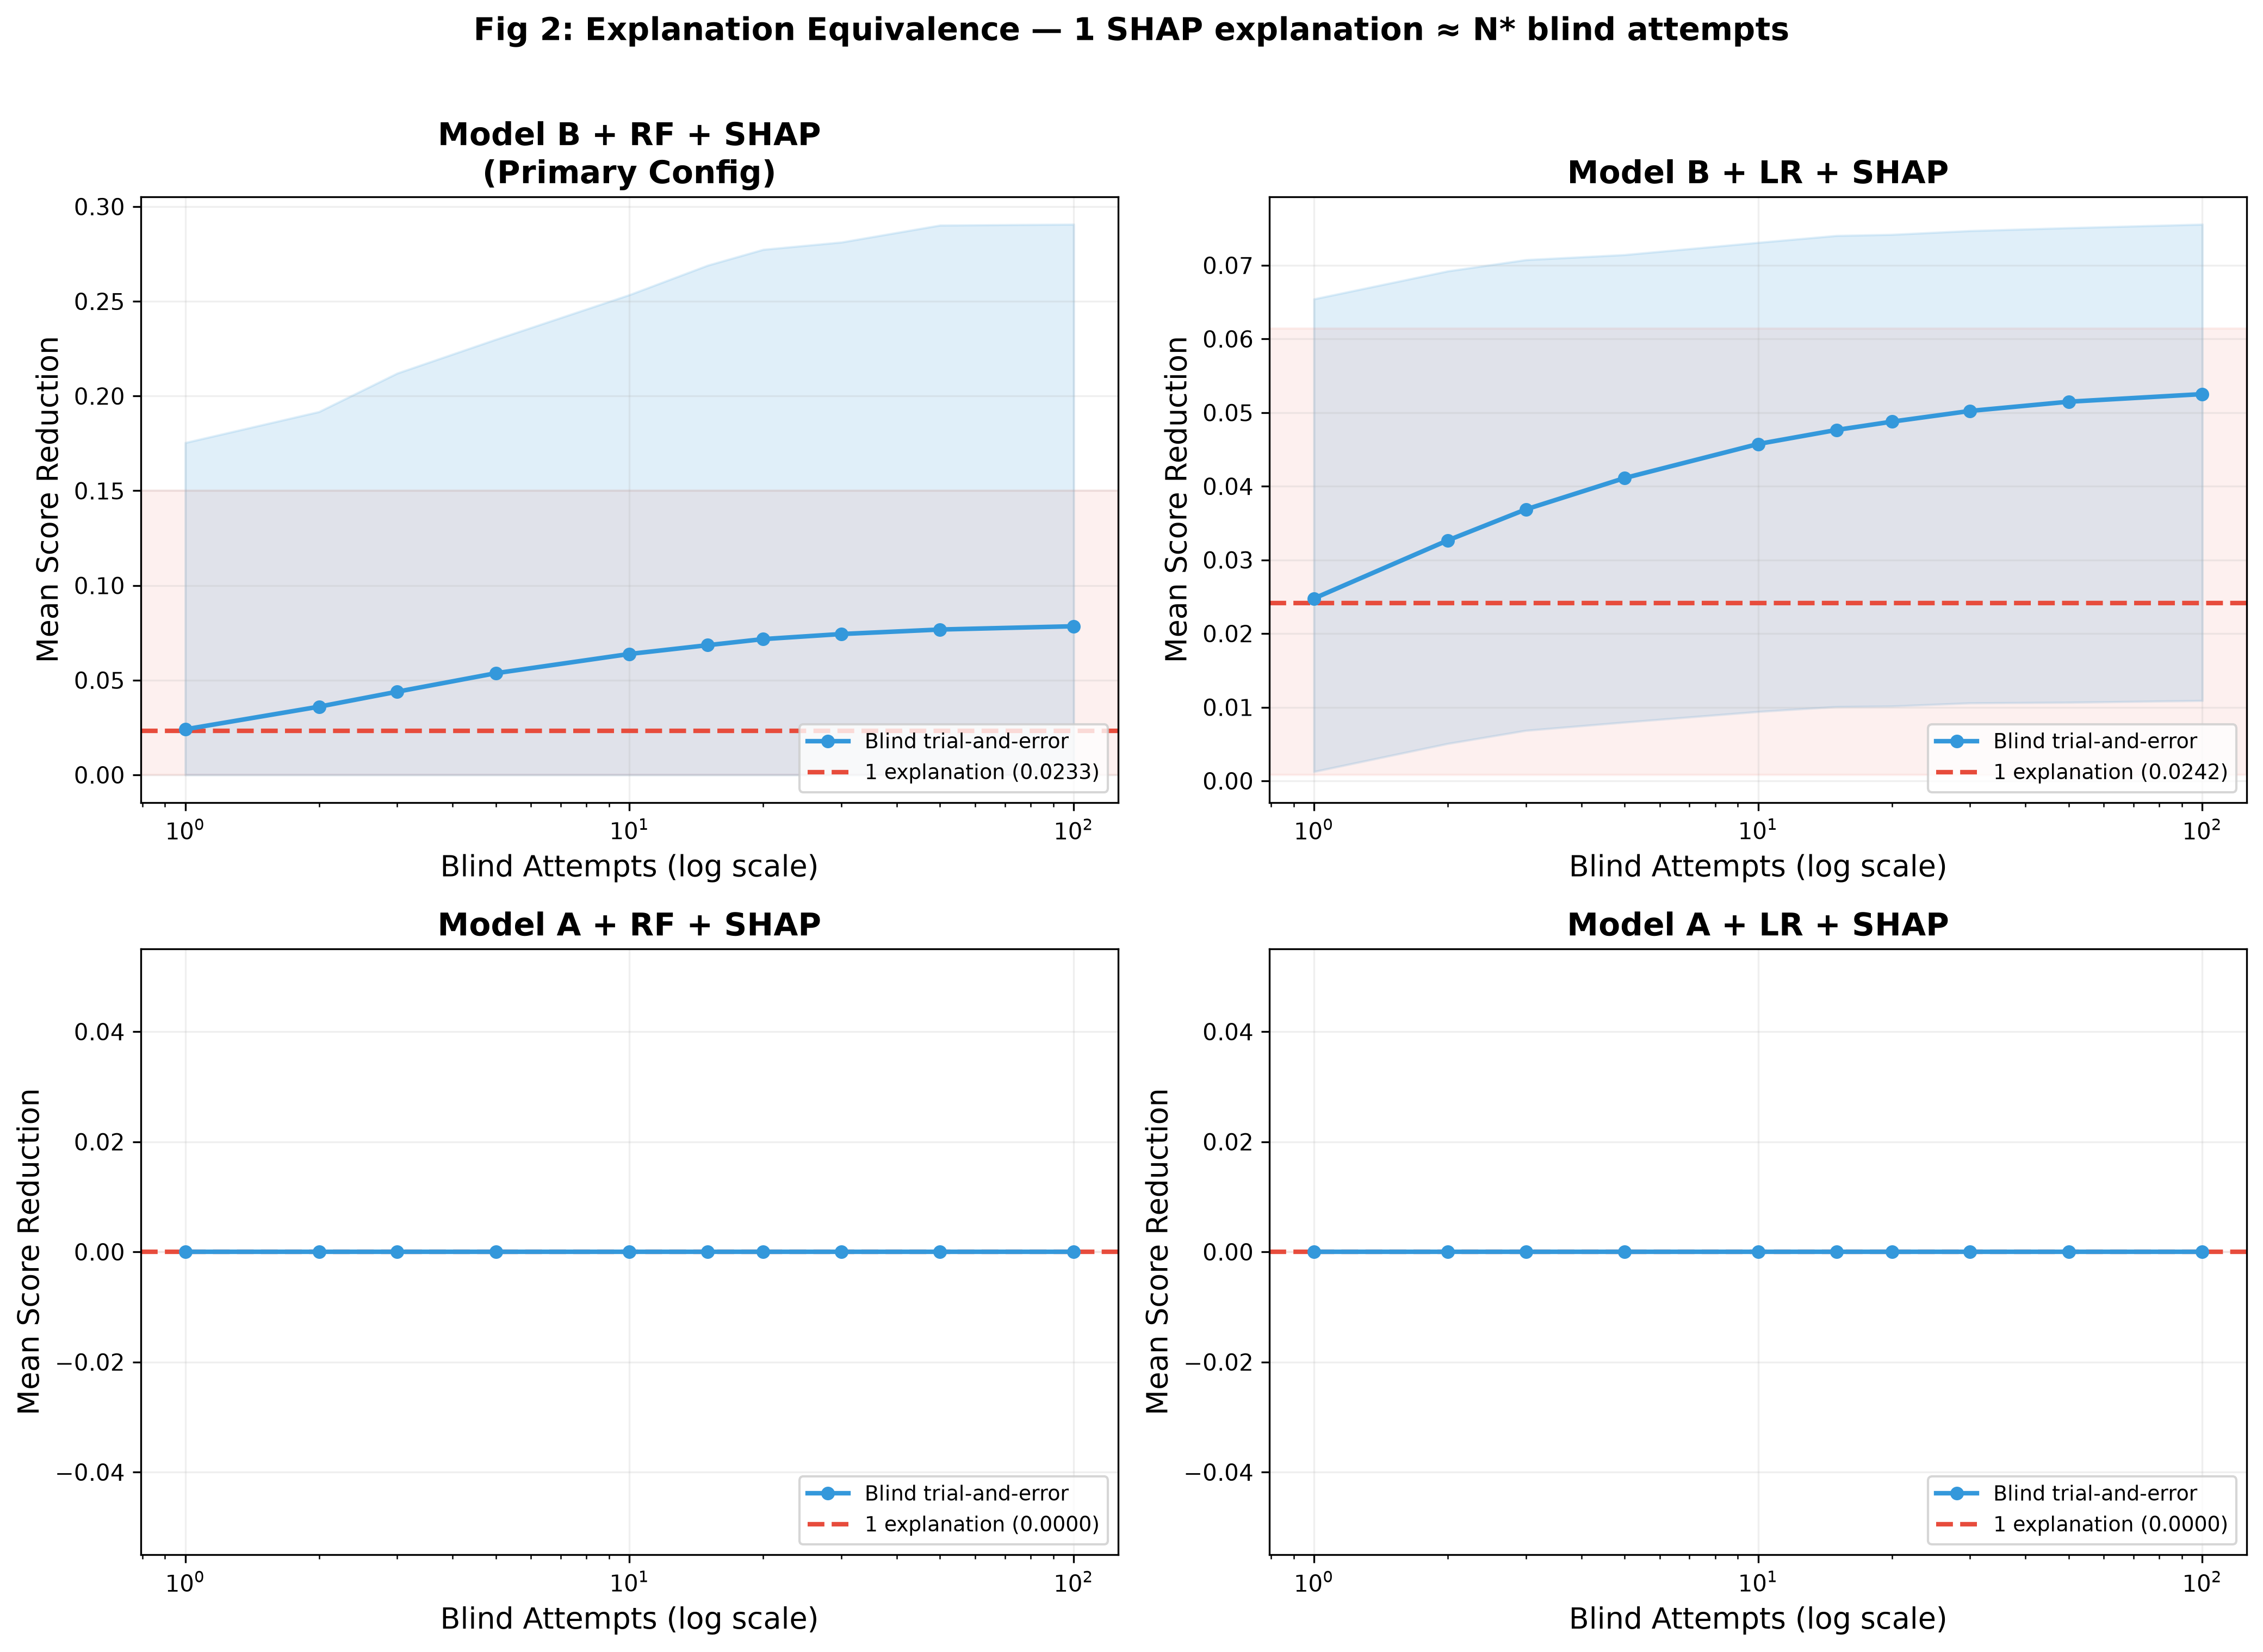
\includegraphics[width=0.85\linewidth]{../results/figures/fig2_main_result.png}
  \caption{Mean score reduction from the best of $N$ blind attempts
           (blue) vs.\ one explanation-guided lie (red dashed), SHAP,
           2017--2018.  For Model B the explanation line does not rise
           above the first blind attempt, so $N^*=0$.  Model A cannot be
           gamed.}
  \label{fig:main_result}
\end{figure*}

\subsection{Why the Explanation Does Not Help More}

With realistic lies the direction is fixed (taller, lighter) and the
lie size is drawn the same way for both strategies, so an explanation
can only tell the patient \emph{which} of height and weight to change;
two or three blind attempts reveal the same.  For the Random Forest the
suggested lie also often backfires: 28.5\% (SHAP) and 31.1\% (LIME) of
explanation-guided lies \emph{raise} the score and are undone, because
local attributions do not describe the model's response over the whole
range of a lie, the practical face of the impossibility result of
Bilodeau et al.~\cite{bilodeau2024impossibility}.  For the Logistic
Regression, whose response is monotone, no SHAP-guided lie backfires.
The two late corrections (undoing a bad lie; reading SHAP relative to
the average patient) raised the primary configuration's explanation
reduction from 0.013 to 0.018 to 0.023, against 0.024 for one blind
attempt, without changing $N^*$
(\texttt{docs/preregistration\_disclosure.md}).

\subsection{Per-Patient Distribution}

Per patient (\cref{fig:hist}), the explanation is no better than one
blind attempt for 69.6\% of patients (RF+SHAP) and worth 10 or more
attempts for 9.5\% (6.7\% beat all 100 attempts).  The per-patient mean
$N^*$ (7.8 for RF+SHAP, 3.6 for LR+SHAP) is therefore driven by a
small tail.

\begin{figure}[t]
  \centering
  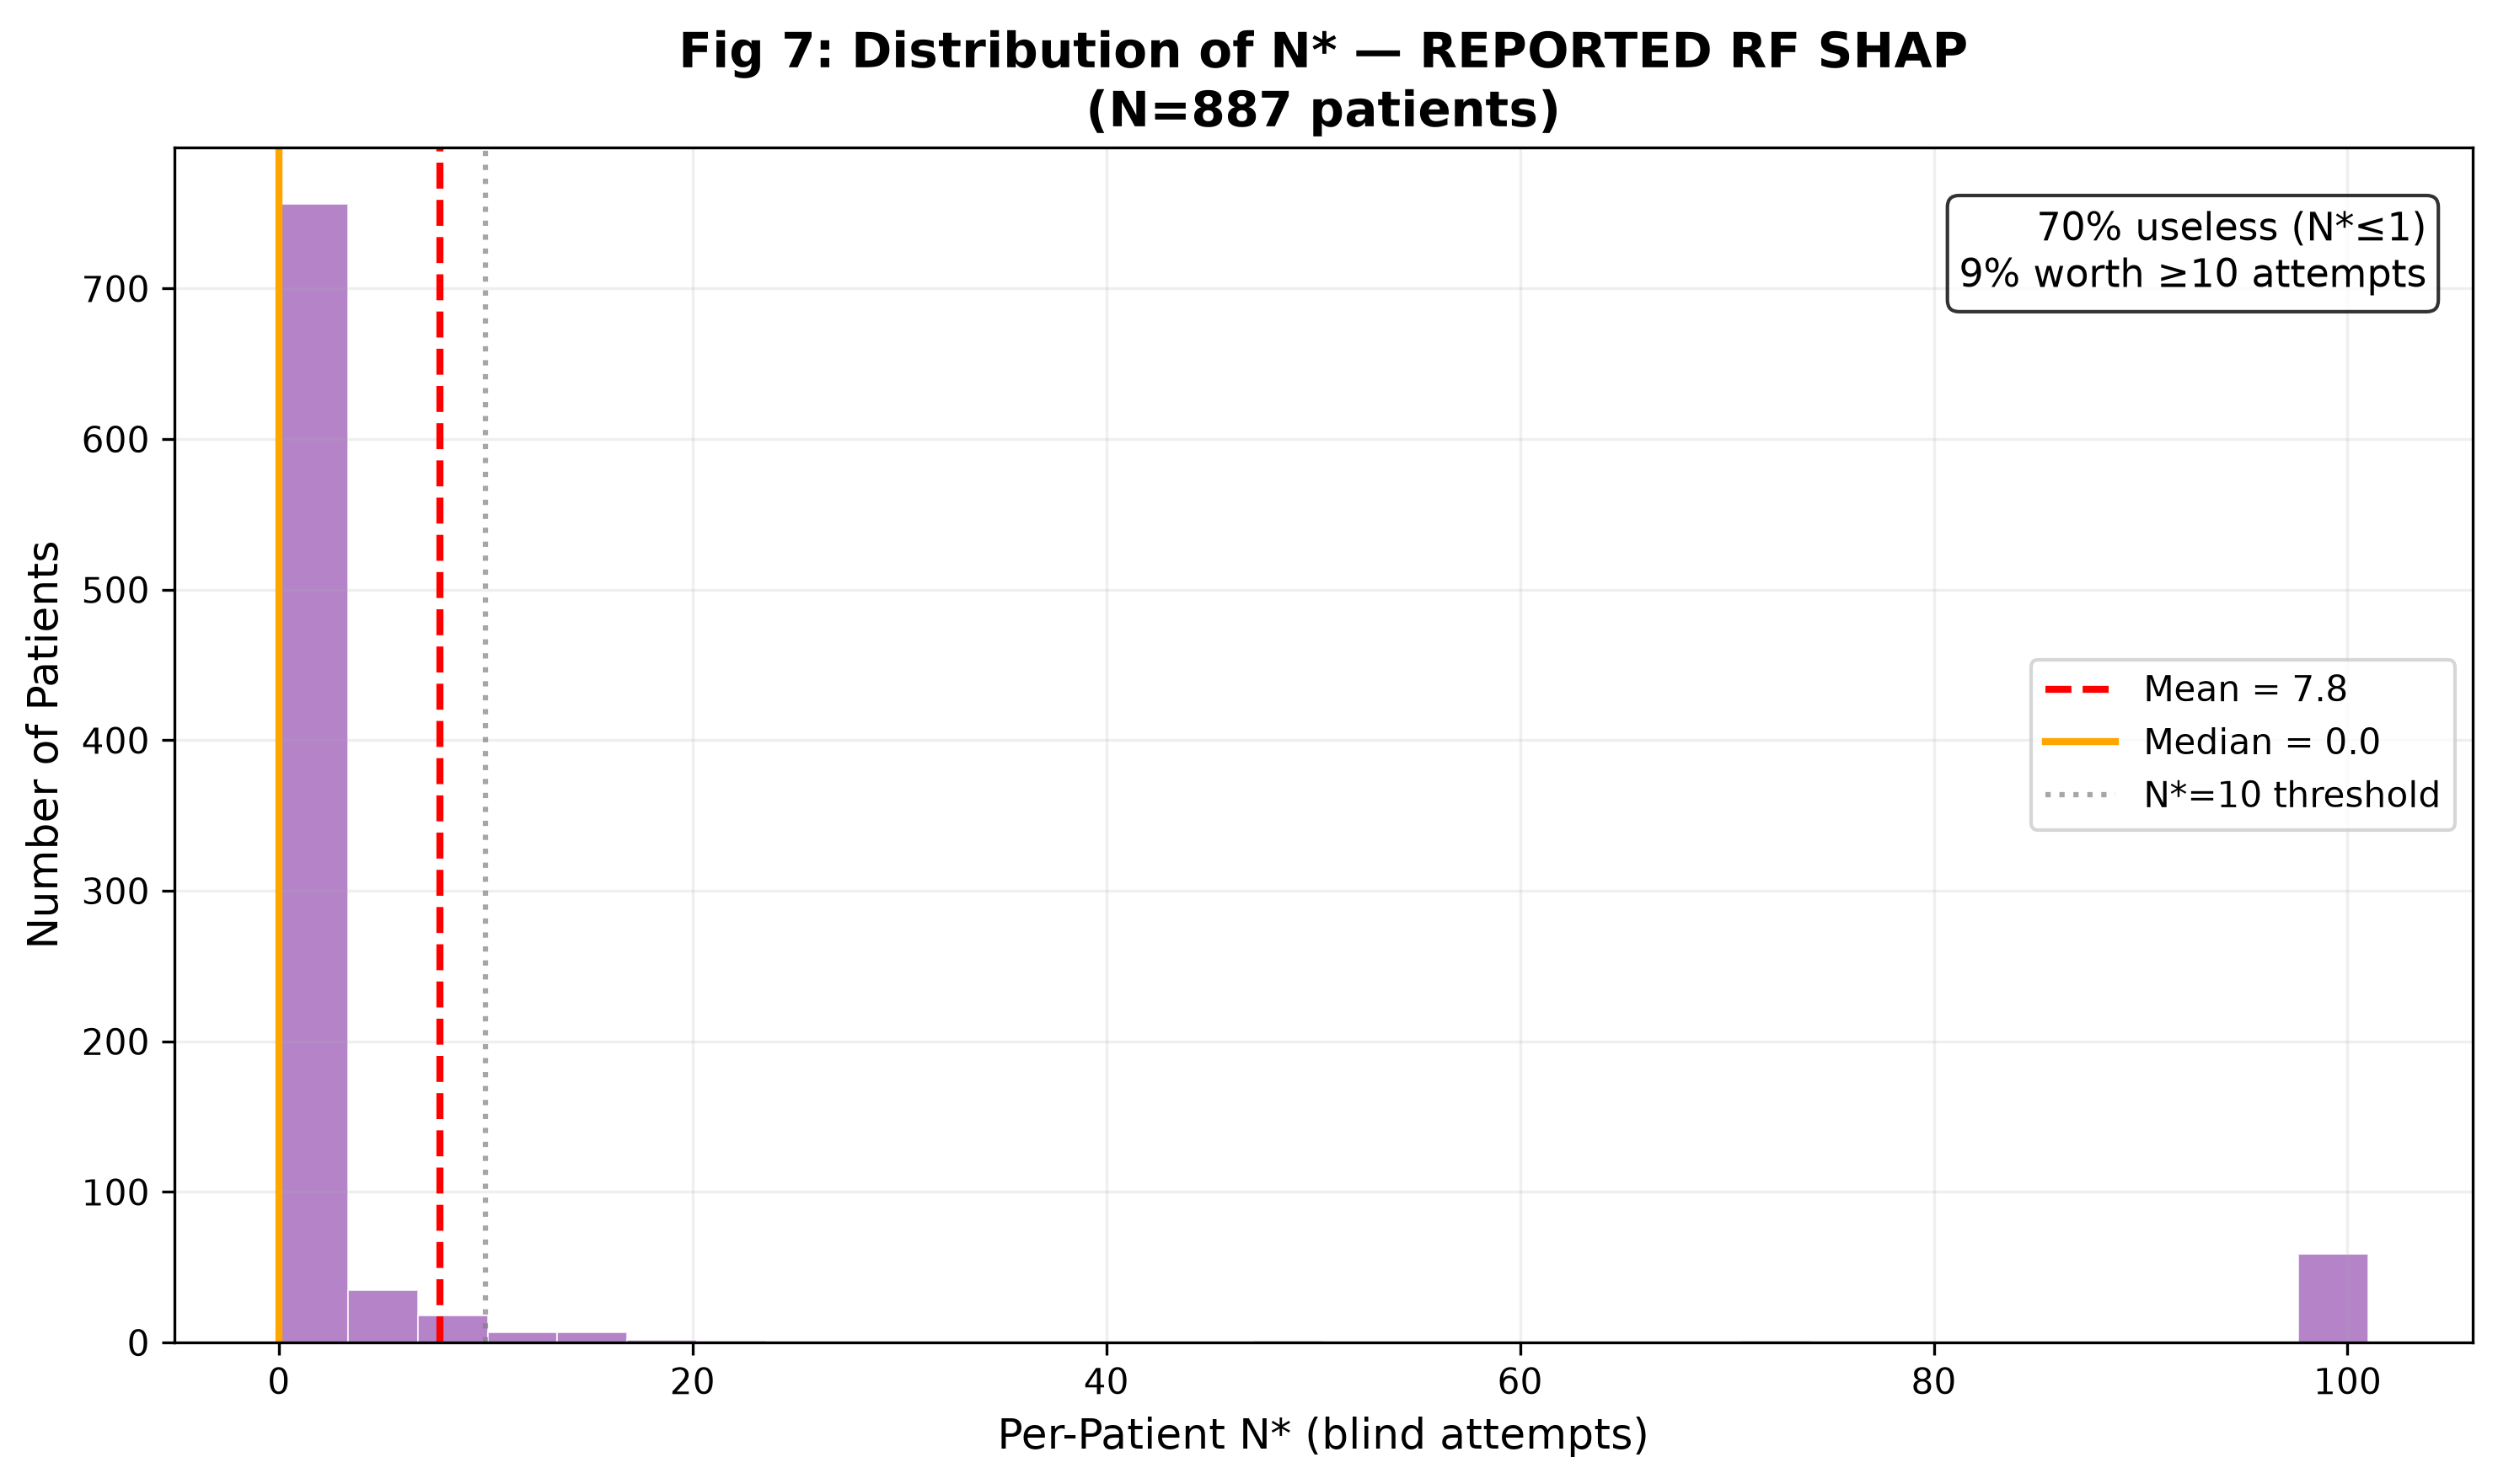
\includegraphics[width=\linewidth]{../results/figures/fig7_nstar_histogram.png}
  \caption{Distribution of per-patient $N^*$ (Model B, RF + SHAP;
           $n=887$ patients, 2017--2018).}
  \label{fig:hist}
\end{figure}

\subsection{Model A vs.\ Model B}

That Model A cannot be gamed is true \emph{by design}: its height and
weight come from the nurse, so it has no input the patient can change,
and its zeros in \cref{tab:model_ab} follow from the threat model rather
than from the experiment.  The measurable comparison has two parts.
Model B, which differs only in using self-reported values, can be
lowered by 0.046--0.064 with ten blind attempts and 0.053--0.079 with a
hundred (\cref{fig:modelab}).  And using measured instead of
self-reported inputs changes accuracy by an amount indistinguishable
from zero on the same test patients (\cref{tab:input_source}): AUC
difference $+0.005$ for RF (95\% CI $-0.009$ to $+0.018$) and $-0.006$
for LR ($-0.013$ to $+0.000$).  Verifying the two self-reported inputs
removes the attack surface at no measurable cost in accuracy.

\begin{figure}[t]
  \centering
  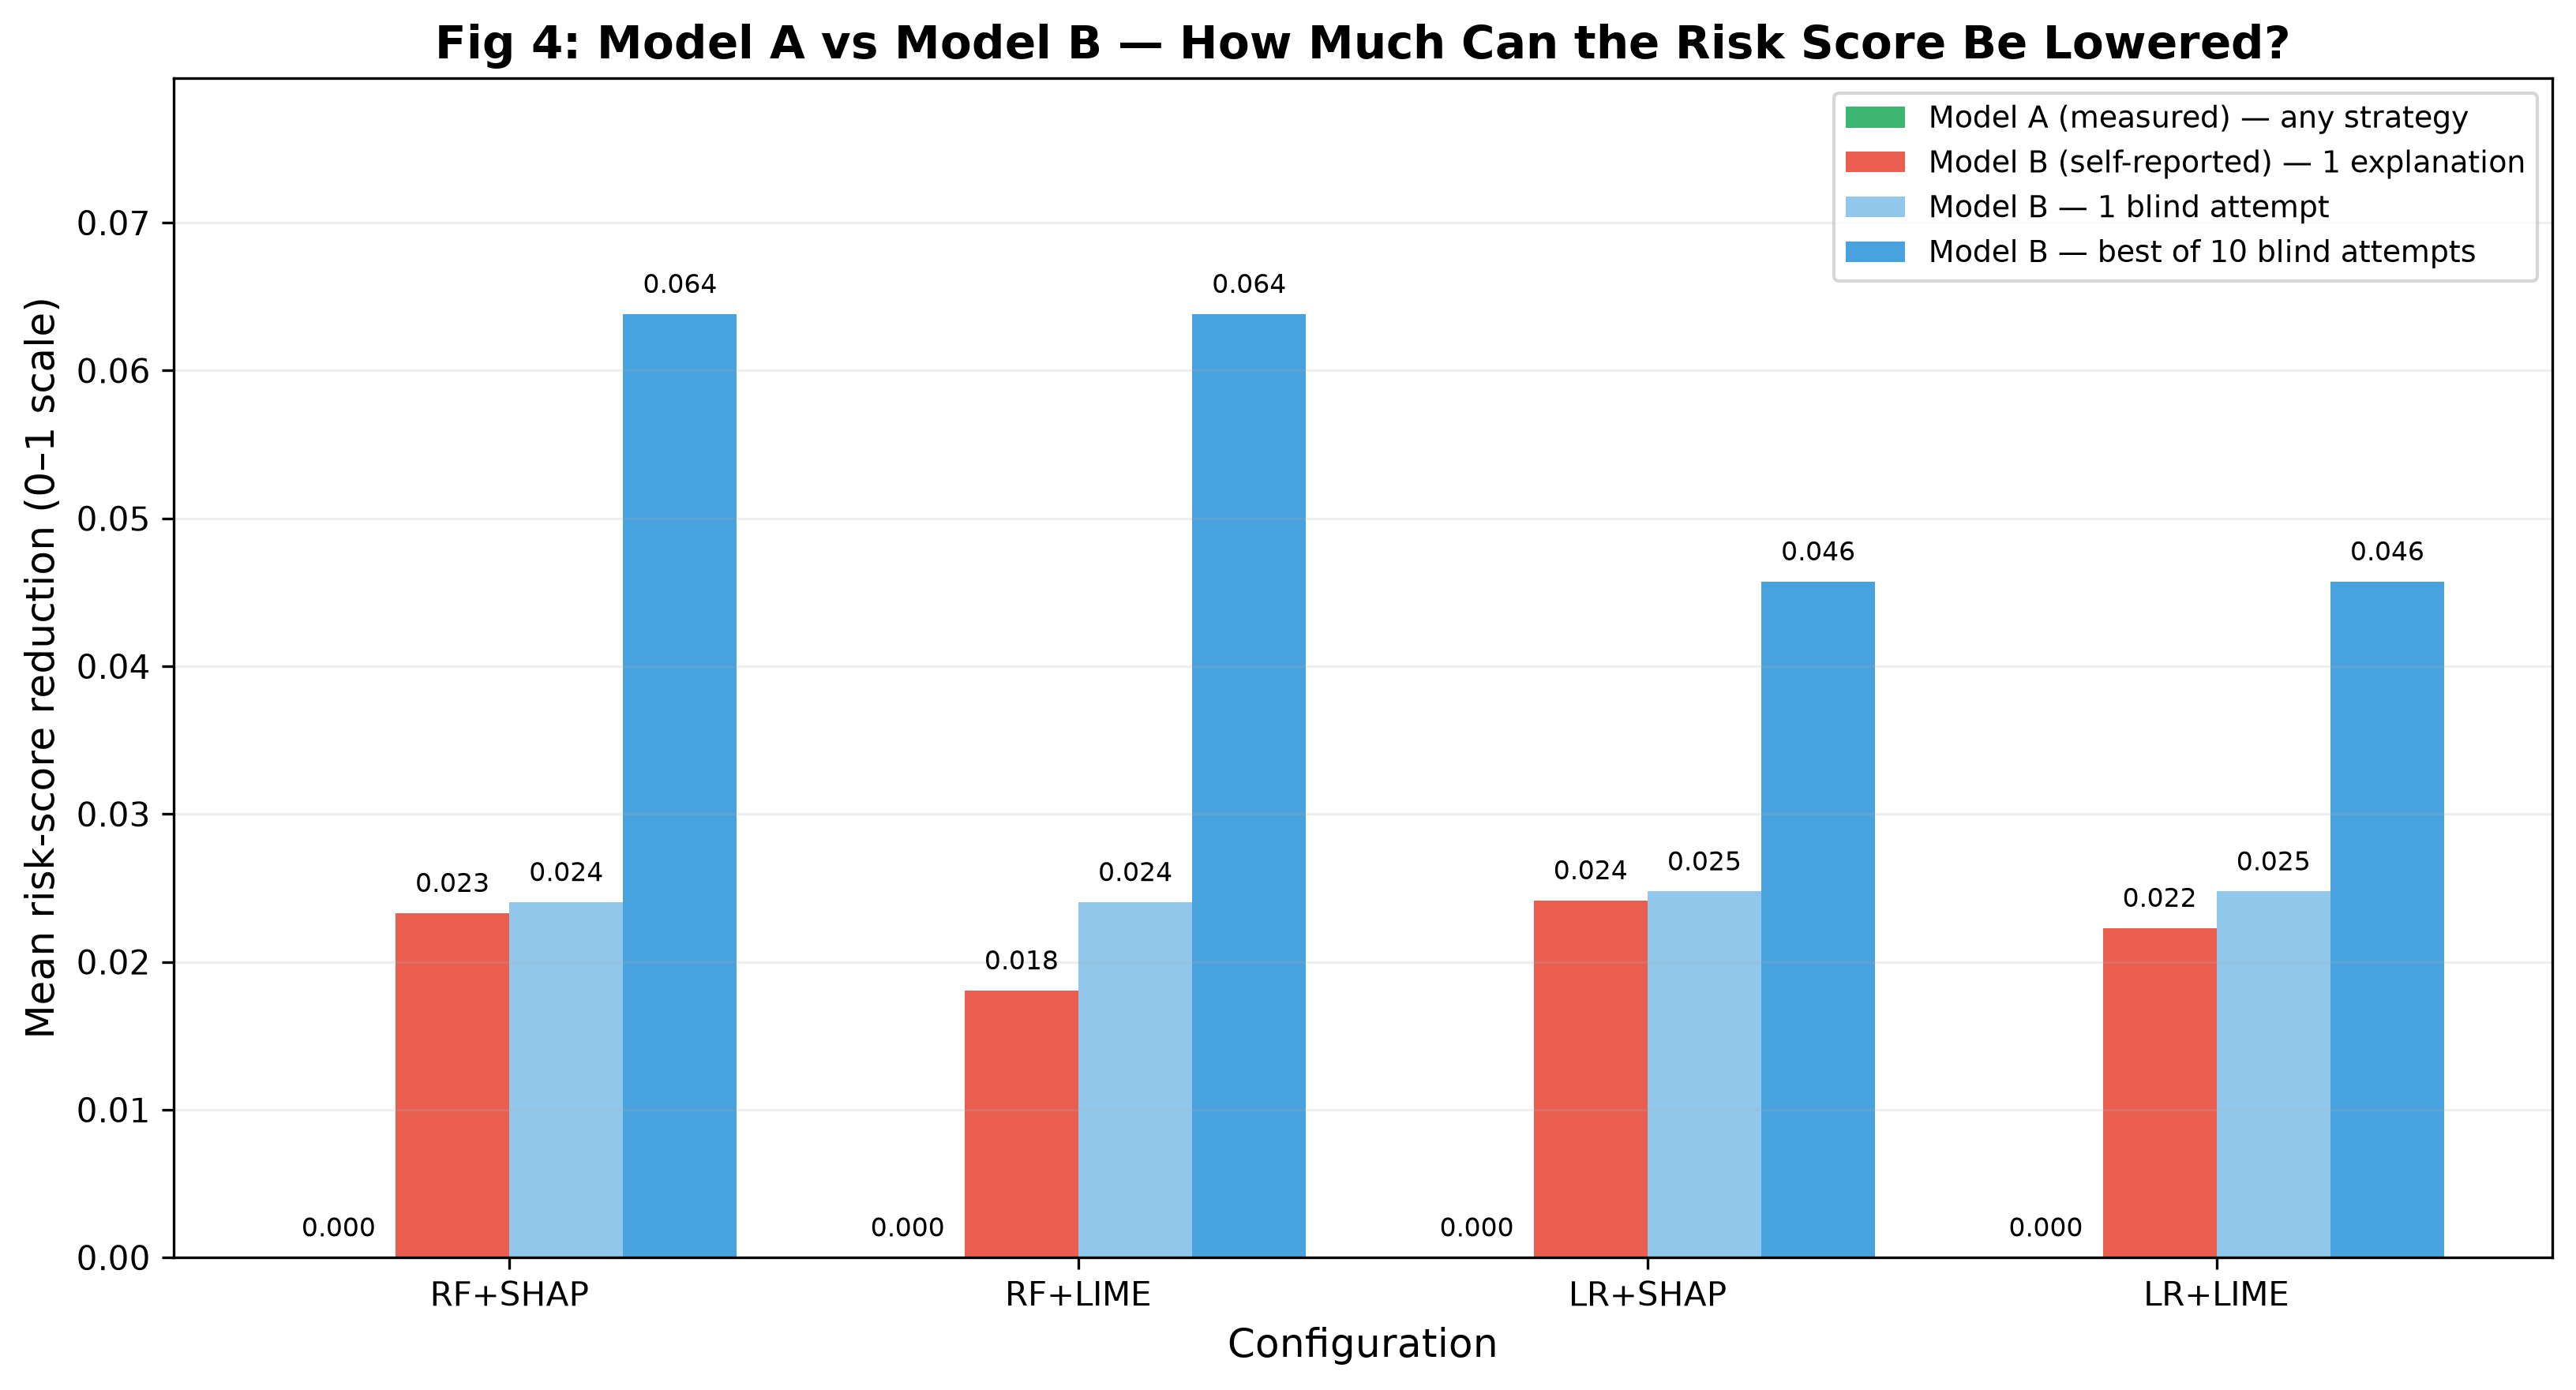
\includegraphics[width=\linewidth]{../results/figures/fig4_model_comparison.png}
  \caption{Mean risk-score reduction for Model A (nurse-measured
           inputs) and Model B (self-reported inputs).}
  \label{fig:modelab}
\end{figure}

\begin{table*}[htbp]
  \centering
  \caption{Model A (Measured) vs Model B (Self-Reported): Vulnerability Comparison}
  \label{tab:model_ab}
  \small
  \resizebox{\ifdim\width>\linewidth\linewidth\else\width\fi}{!}{%
  \begin{tabular}{lrrrrrr}
    \toprule
    Config & Model A $N^*$ & Model B $N^*$ & A: reduction, 10 blind & B: reduction, 1 explanation & B: reduction, 10 blind & B can be gamed \\
    \midrule
    RF+SHAP & 0.0 & 0.0 & 0.0 & 0.0129 & 0.0638 & Yes \\
    RF+LIME & 0.0 & 0.0 & 0.0 & 0.0117 & 0.0638 & Yes \\
    LR+SHAP & 0.0 & 0.0 & 0.0 & 0.0176 & 0.0457 & Yes \\
    LR+LIME & 0.0 & 0.0 & 0.0 & 0.0223 & 0.0457 & Yes \\
    \bottomrule
  \end{tabular}%
  }
\end{table*}


\begin{table*}[htbp]
  \centering
  \caption{Self-reported vs measured height/weight on the same patients: accuracy difference (Model A minus Model B, paired bootstrap 95\% CI) and how far Model B can be gamed. Model A cannot be gamed by construction.}
  \label{tab:input_source}
  \small
  \resizebox{\ifdim\width>\linewidth\linewidth\else\width\fi}{!}{%
  \begin{tabular}{lrrrrr}
    \toprule
    Model & AUC A (measured) & AUC B (self-reported) & Difference A-B & 95\% CI (paired bootstrap) & B: max reduction, 10 blind lies \\
    \midrule
    RF & 0.7981 & 0.7933 & 0.0047 & [-0.0093, +0.0177] & 0.0638 \\
    LR & 0.7734 & 0.7796 & -0.0062 & [-0.0127, +0.0002] & 0.0457 \\
    \bottomrule
  \end{tabular}%
  }
\end{table*}


\subsection{SHAP vs.\ LIME Agreement}

Because each patient receives the same lie size under SHAP and LIME,
differences come from the explanation alone (\cref{fig:scatter}).  The
two methods lead to the same outcome for 74\% (RF) and 71\% (LR) of
patients, with per-patient correlation $r = 0.65$ and $0.87$.  Both
give $N^*=0$; SHAP is slightly better than LIME (RF 0.023 vs.\ 0.018;
LR 0.024 vs.\ 0.022).

\begin{figure*}[t]
  \centering
  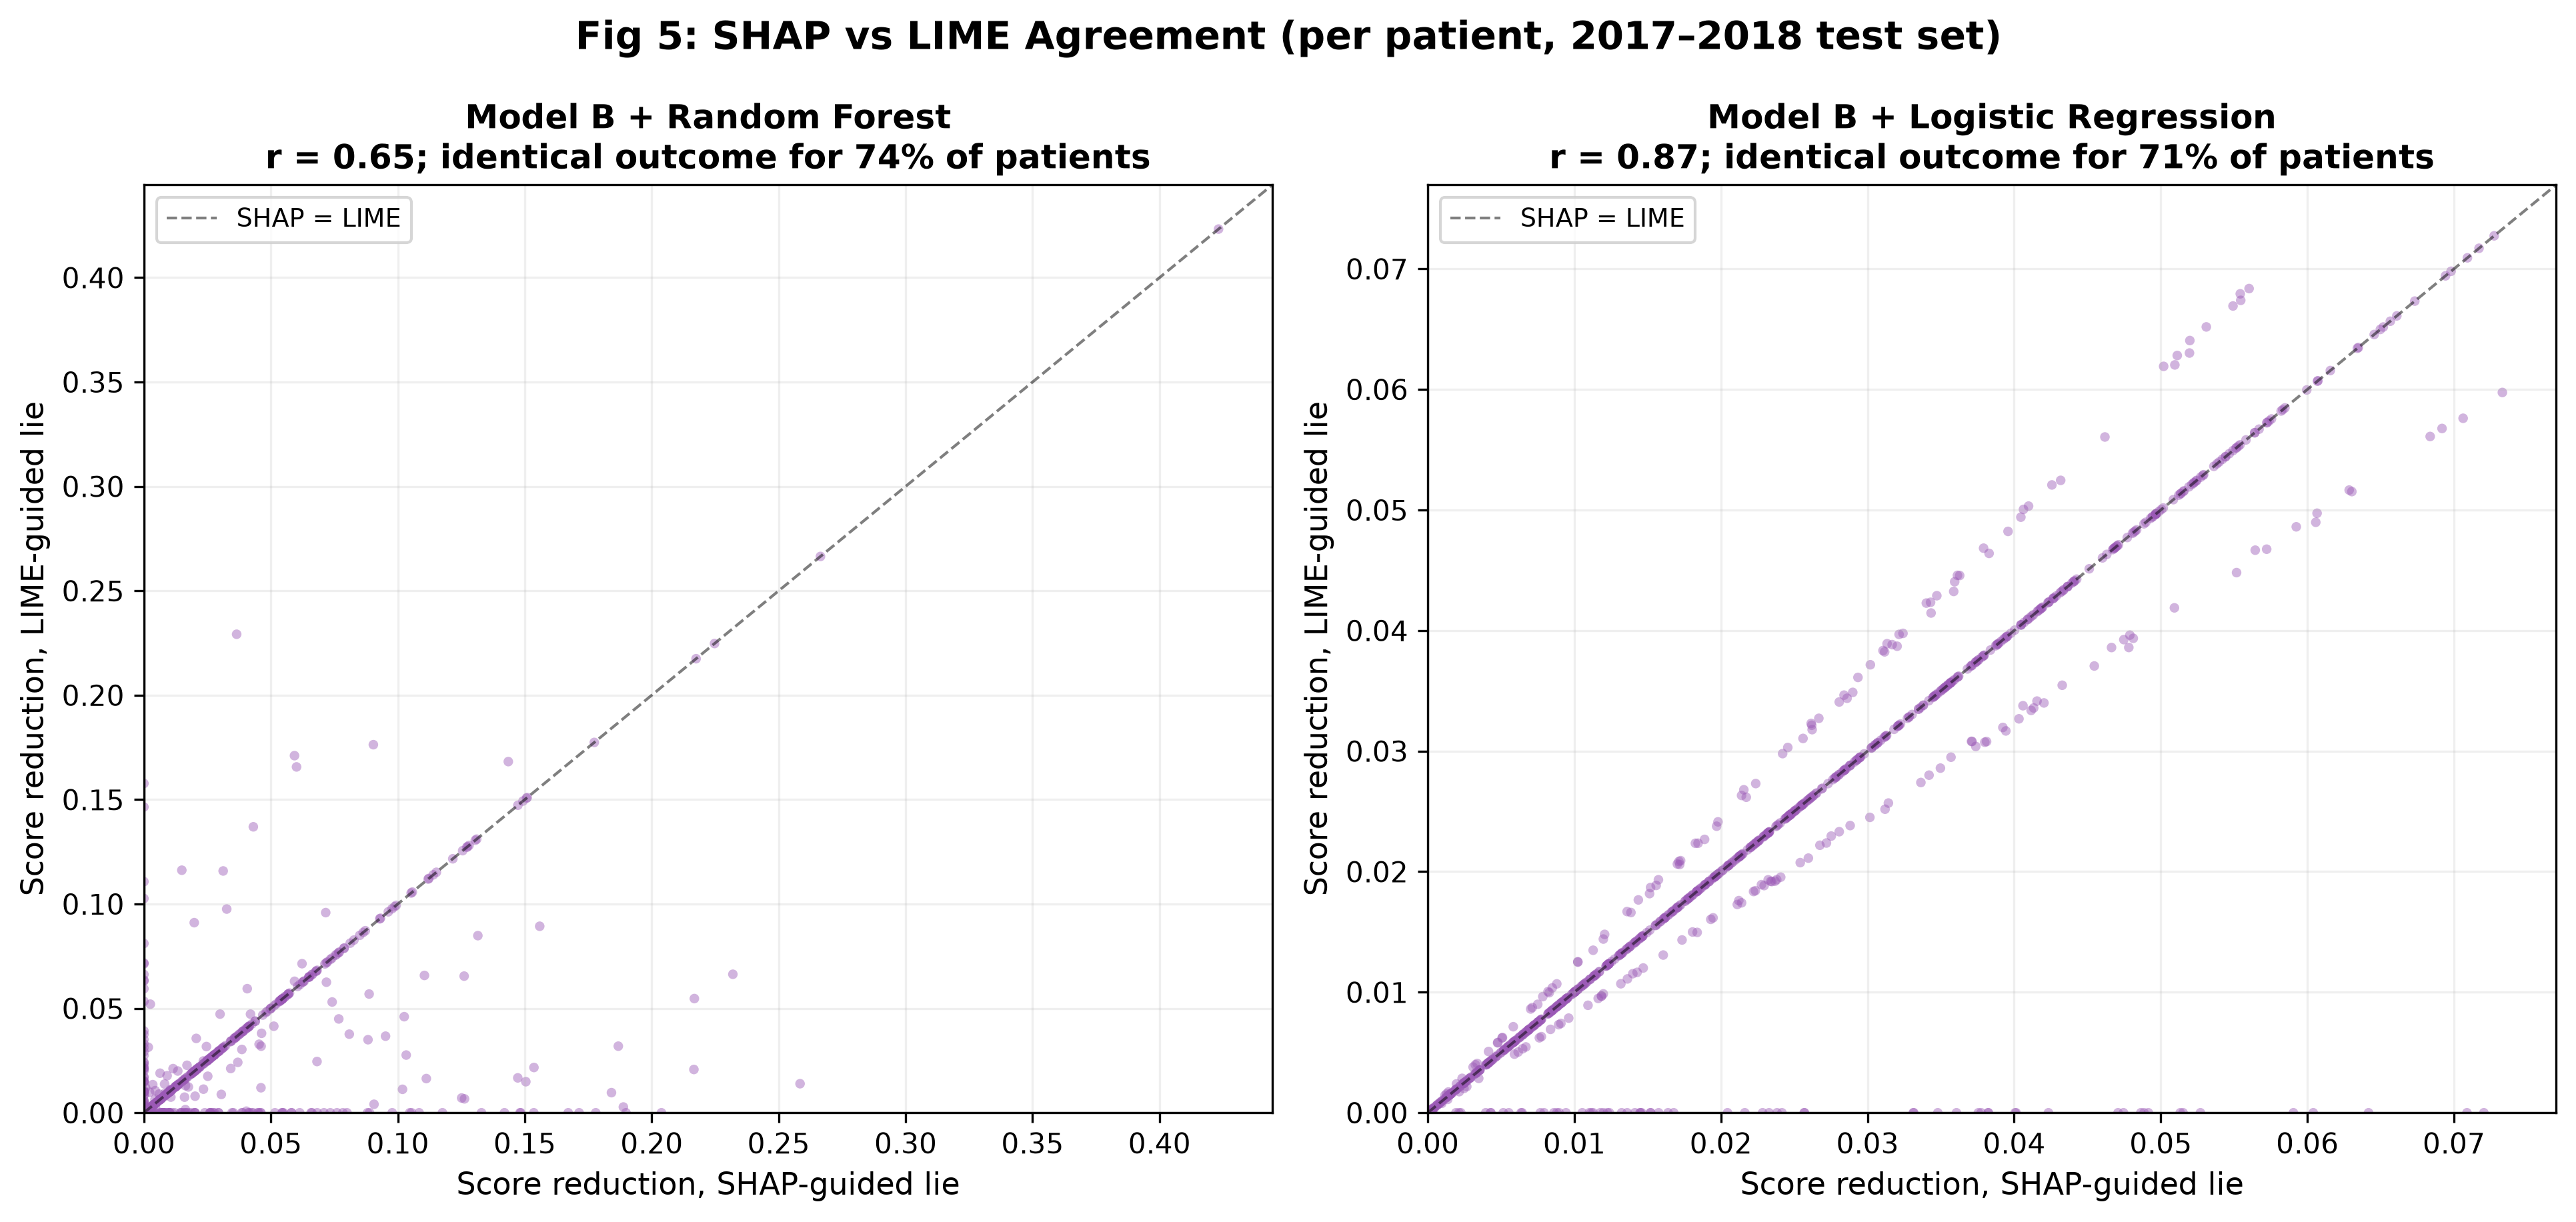
\includegraphics[width=0.85\linewidth]{../results/figures/fig5_shap_lime_scatter.png}
  \caption{Per-patient score reduction from the SHAP-guided lie vs.\
           the LIME-guided lie (Model B, 2017--2018 test set).}
  \label{fig:scatter}
\end{figure*}

\subsection{Statistical Tests}

The one-sided Wilcoxon test of explanation $>$ blind at $N=10$ is not
significant in any configuration ($p = 1.0$, also after Holm
correction; \cref{tab:stats}).  The effect sizes are large and
\emph{negative} ($d = -0.66$ to $-1.24$ for Model B): ten blind
attempts lower the score clearly more than one explanation.

\begin{table}[htbp]
  \centering
  \caption{Statistical Tests: Explanation vs Blind (N=10), Wilcoxon Signed-Rank}
  \label{tab:stats}
  \small
  \begin{tabular}{lrrr}
    \toprule
    Config & Wilcoxon p & Cohen's d & Significant \\
    \midrule
    reported\_rf\_shap & 1.000000 & -0.801 & No \\
    reported\_rf\_lime & 1.000000 & -0.789 & No \\
    reported\_lr\_shap & 1.000000 & -1.336 & No \\
    reported\_lr\_lime & 1.000000 & -1.238 & No \\
    measured\_rf\_shap & 1.000000 & 0.000 & No \\
    measured\_rf\_lime & 1.000000 & 0.000 & No \\
    measured\_lr\_shap & 1.000000 & 0.000 & No \\
    measured\_lr\_lime & 1.000000 & 0.000 & No \\
    \bottomrule
  \end{tabular}
\end{table}


\subsection{Comparison Dataset: CDC Diabetes Health Indicators}

On 1{,}000 sampled test respondents of BRFSS 2015 (UCI 891), with
self-reported BMI as the only gameable feature, the result is the same
(\cref{tab:uci891}): $N^* = 0.0$ in all four configurations (upper CI
bound at most 1.1); one explanation-guided lie lowers the score by
0.026--0.041 against 0.037--0.044 for one blind attempt.  BRFSS has no
measured BMI and a self-reported diabetes label, so this supports only
the Model~B finding, with a BMI lie budget borrowed from NHANES.

\begin{table*}[t]
  \centering
  \caption{Comparison dataset (CDC Diabetes Health Indicators, UCI 891; BRFSS 2015, 1{,}000 sampled test respondents): one explanation vs.\ blind attempts, with self-reported BMI as the only gameable feature.}
  \label{tab:uci891}
  \small
  \resizebox{\linewidth}{!}{%
  \begin{tabular}{llrrrrrrrrrrr}
    \toprule
    Model & Expl. & N & N* & N* 95\% CI & 1 explanation & 1 blind & 10 blind & Per-patient mean N* & \% useless & \% lie undone & Wilcoxon p & Cohen's d \\
    \midrule
    RF & SHAP & 1000 & 0.0 & [0.00, 1.04] & 0.0409 & 0.0436 & 0.0772 & 16.98 & 67.8 & 16.5 & 1.0 & -0.703 \\
    RF & LIME & 1000 & 0.0 & [0.00, 0.00] & 0.0324 & 0.0436 & 0.0772 & 13.86 & 74.7 & 13.6 & 1.0 & -0.829 \\
    LR & SHAP & 1000 & 0.0 & [0.00, 1.12] & 0.0369 & 0.0373 & 0.0655 & 4.04 & 49.8 & 0.0 & 1.0 & -1.142 \\
    LR & LIME & 1000 & 0.0 & [0.00, 0.00] & 0.0257 & 0.0373 & 0.0655 & 2.85 & 63.8 & 0.0 & 1.0 & -1.316 \\
    \bottomrule
  \end{tabular}}
\end{table*}


\subsection{Confirmatory Result: NHANES 2021--2023}
\label{sec:confirmatory-results}

The confirmatory run used the code and settings fixed at the
\texttt{v0.2-preregistration} tag (commit \texttt{5b2f240}), unchanged,
on NHANES August 2021--August 2023: 5{,}628 adults with complete data
(11.9\% with diabetes) and 1{,}126 test patients.  The reporting gap was
again stable (height $+1.73$\,cm, weight $-0.65$\,kg on average;
95th percentiles 6.84\,cm and 9.04\,kg against the 7.28\,cm and
8.96\,kg budget used).

\begin{table*}[t]
  \centering
  \caption{Confirmatory result, NHANES 2021--2023 (pre-registered,
           $n = 1{,}126$ test patients). Mean score reductions; Model A
           (measured) is 0 in every column by design.}
  \label{tab:confirmatory}
  \small
  \begin{tabular}{lrcrrrr}
    \toprule
    Model B config & $N^*$ & 95\% CI & 1 expl. & 1 blind & 10 blind & Cohen's $d$ \\
    \midrule
    RF + SHAP (primary) & 1.42 & [1.21, 1.62] & 0.034 & 0.028 & 0.070 & $-0.71$ \\
    RF + LIME & 0.00 & [0.00, 0.00] & 0.024 & 0.028 & 0.070 & $-0.76$ \\
    LR + SHAP & 1.07 & [0.00, 1.20] & 0.035 & 0.035 & 0.062 & $-1.14$ \\
    LR + LIME & 0.00 & [0.00, 0.00] & 0.032 & 0.035 & 0.062 & $-1.19$ \\
    \bottomrule
  \end{tabular}
\end{table*}

For the primary configuration, $N^* = 1.42$ (95\% CI 1.21--1.62): one
SHAP explanation is worth about one and a half blind attempts, inside
the pre-registered ``minimal advantage'' band ($N^* < 5$), and the
upper confidence bound is far below 5 (\cref{tab:confirmatory}).
Across Model~B, $N^*$ ranges from 0 to 1.42; the one-sided Wilcoxon
test of explanation $>$ ten blind attempts is not significant in any
configuration ($p = 1.0$, also after Holm correction), with large
negative effect sizes.  Every pre-registered prediction held.  As in
2017--2018, Random Forest lies suggested by an explanation backfired
for 27\% of patients.  Unlike 2017--2018, SHAP now does slightly
\emph{better} than one blind attempt (0.034 vs.\ 0.028 for the Random
Forest), which is why $N^*$ is above zero; LIME does not.

Model~A again cannot be gamed.  The accuracy difference between
measured and self-reported inputs on the same test patients is $+0.006$
for the Random Forest (95\% CI $-0.014$ to $+0.026$) and $-0.012$ for
the Logistic Regression ($-0.023$ to $-0.002$), i.e.\ in this cycle the
self-reported Logistic Regression is slightly \emph{more} accurate.
Either way the difference is about one hundredth of AUC, small against
the 0.06--0.07 by which ten blind lies lower a Model~B score.

% ============================================================
\section{Discussion}
% ============================================================

\subsection{Policy Implications}

Our pre-registered interpretation guide set three bands: $N^*<5$
(withholding explanations is not a meaningful safeguard),
$5 \le N^* \le 20$ (moderate advantage), and $N^*>20$ (explanations are
powerful attack vectors).  With $N^* \le 1.42$ in every configuration
of the confirmatory test (upper CI bound 1.62), the result falls in the
first band.  Under realistic lies, an explanation
does not give a patient a better route to a lower score than simply
trying an answer; withholding it would remove information from honest
users while barely slowing a motivated one.  The vulnerability lies
in the self-reported inputs: the measured-input model cannot be gamed,
and the two models are equally accurate.

This conclusion runs against the intuition that explanations are
``instructions for cheating''.  The reason is that a feature
attribution answers ``what contributed to this score?'', not ``what
should I change?'', and the two can point in different directions.

\subsection{Limitations}

\begin{itemize}
  \item \textbf{Model of the patient.} We model one way of reading an
        explanation (follow the top realistic suggestion once).  A
        more sophisticated reader, or a counterfactual explanation,
        could extract more.
  \item \textbf{Single lie, single feature.} Each explanation-guided
        attempt changes one feature once; multi-feature lies could be
        more powerful for both strategies.
  \item \textbf{Lie model.} Lie size is uniform within the
        95th-percentile gap and in the observed direction, so an
        explanation can only choose \emph{which} feature to change.
        Using the maximum lie, or allowing either direction, is a
        one-line change in our code; we leave that sensitivity analysis
        to future work.
  \item \textbf{Domain.} Results are for diabetes risk from
        anthropometric self-report (NHANES, and BRFSS as a comparison
        whose diabetes label is itself self-reported).
  \item \textbf{Survey changes.} In 2021--2023 blood pressure is
        measured oscillometrically and the activity question was
        redesigned; we mapped both before seeing the data.
  \item \textbf{Pre-registration and deviations.} The plan was
        recorded as a git tag in the project repository rather than an
        independent registry; a first run on the 2017--2018 data was
        seen before the analysis was corrected, and eight settings
        deviate from the first plan (\cref{sec:preregistration}).  We
        therefore treat 2017--2018 as exploratory and rest our
        conclusion on the re-registered 2021--2023 test.
\end{itemize}

\subsection{Recommendations for Practitioners}

\begin{enumerate}
  \item Prefer \textbf{verified inputs} (e.g.\ nurse measurement) over
        self-report for the features that drive high-stakes predictions.
  \item Do not withhold explanations as an anti-gaming measure; audit
        the gain they give with the $N^*$ framework.
  \item Be aware that attributions are not advice: present them as
        ``contributions'' rather than ``what to change''.
\end{enumerate}

% ============================================================
\section{Conclusion}
% ============================================================

We introduced the \emph{explanation equivalence} metric $N^*$ and
applied it to a diabetes risk model using real NHANES survey data,
with lies bounded by how people actually misreport.  In a
pre-registered confirmatory test on unseen NHANES 2021--2023 data, one
SHAP or LIME explanation was worth at most about one and a half blind
attempts ($N^* = 1.42$, 95\% CI 1.21--1.62, for the primary
configuration; 0--1.42 overall), and an exploratory 2017--2018 analysis
and a second survey agreed.  For the Random Forest, explanation-guided
lies often raised the score instead.  A model using nurse-measured
inputs could not be gamed and was as accurate.  The effective
safeguard against gaming is therefore verifying self-reported inputs,
not withholding explanations.

\paragraph{Future Work.}
Sensitivity to the lie model, multi-feature and multi-step attacks,
counterfactual explanations, other clinical domains, and a user study
of how real patients read explanations.

\paragraph{Code and Data.}
Code, analysis plan and results:
\url{https://github.com/AkkiNikumbh/BTECH_PROJECT}.  NHANES data are
public and are downloaded by the pipeline.

% ============================================================
% REFERENCES
% ============================================================

\bibliographystyle{ACM-Reference-Format}
\bibliography{references}

\end{document}
